% -*- latex -*-
%
% The SAND document class is maintained at:
%
%    http://www.cs.sandia.gov/SANDreport
%
% This page also has instructions and documentation on commands.
%
\documentclass[12pt,report]{SANDreport}

\SANDnum{SAND20XX-XXXX}
\SANDprintDate{January 20XX}

\title{VTK-m Users' Guide \\
  \relsize{-2}Version 0.0
}
\author{Kenneth~Moreland \\
  \relsize{-2} Scalable Analysis and Visualization \\[-1ex]
  \relsize{-2} Sandia National Laboratories \\[-1ex]
  \relsize{-2} P.O. Box 5800 MS 1323 \\[-1ex]
  \relsize{-2} Albuquerque, NM 87185-1323 \\[-1ex]
  \relsize{-2} kmorel@sandia.gov
}
\SANDauthor{Kenneth~Moreland}
\date{} % Leave empty


\usepackage{amsfonts}
\usepackage{amssymb}
\usepackage{amsmath}
\usepackage{booktabs}
\usepackage{graphicx}
\usepackage{isomath}
\usepackage{varioref}
\usepackage{fancyvrb}
\usepackage{ifthen}
\usepackage{longtable}
\usepackage{cite}
\usepackage{relsize}
\usepackage{subfig}
\usepackage{xspace}

% This wonderful package allows hyphenation in tt fonts and hyphenation of
% words with underscores in them.
\usepackage[htt]{hyphenat}

% This package defines a tt font that supports boldface (albeit not very
% distinctly). The default package has no boldface for tt fonts.
\usepackage{lmodern}

\usepackage{makeidx}
\makeindex

\usepackage[pdfborder={0 0 0}]{hyperref}
\usepackage{verbatim}

\usepackage{color}
\definecolor{yellow}{rgb}{1,1,0}
\definecolor{black}{rgb}{0,0,0}
\definecolor{ltcyan}{rgb}{.75,1,1}
\definecolor{red}{rgb}{1,0,0}
\definecolor{gray}{rgb}{.6,.6,.6}
\definecolor{darkred}{rgb}{0.5,0,0}
\definecolor{darkgreen}{rgb}{0,0.5,0}

\definecolor{vtkmidentifier}{rgb}{0,0,1}
\definecolor{vtkmnamespace}{rgb}{0.5,0,0}
\definecolor{vtkmmacro}{rgb}{0.5,0,0}
\definecolor{vtkmsignature}{rgb}{0,0.5,0}

\usepackage{listings}
\lstloadlanguages{C,C++}
\lstset{fontadjust=false,basicstyle=\scriptsize\ttfamily}
%% \lstset{numbers=left, numberstyle=\tiny, stepnumber=1, numbersep=2pt}
\lstdefinelanguage{VTKm}{
  morekeywords={struct,class,public,typedef,void,template,return,operator,const,for,int},
  morekeywords={[2]Id,Id2,Id3,Scalar,Tuple,Vector2,Vector3,Vector4,
                   make_Id3,make_Vector2,make_Vector3,make_Vector4,
                   dot,NUM_COMPONENTS,
                   Extent,Extent3,Pair,
                   ExtentPointDimensions,ExtentCellDimensions,
                   ExtentNumberOfPoints,ExtentNumberOfCells,
                   ExtentPointFlatIndexToTopologyIndex,
                   ExtentCellFlatIndexToTopologyIndex,
                   ExtentPointTopologyIndexToFlatIndex,
                   ExtentCellTopologyIndexToFlatIndex,
                   WorkletMapField, WorkletMapCell,
                   WorkletGenerateTopology, WorkletInterpolatedCell,
                   WorkletGenerateKeysValues, WorkletReduceKeysValues,
                   ExecutionObjectBase,
                   TypeTraits,NumericTag,DimensionalityTag,
                   TypeTraitsRealTag,TypeTraitsIntegerTag,
                   TypeTraitsScalarTag,TypeTraitsVectorTag,
                   VectorTraits,ComponentType,HasMultipleComponents,
                   VectorTraitsTagMultipleComponents,
                   VectorTraitsTagSingleComponent,
                   Error, ErrorExecution, ErrorControl,
                   ErrorControlAssert, ErrorControlBadValue,
                   ErrorControlInternal, ErrorControlOutOfMemory,
                   DeviceAdapterTagSerial,
                   DeviceAdapterTagCuda,
                   DeviceAdapterTagOpenMP,
                   DeviceAdapterTagTBB,
                   CellAverage,
                   CellDataToPointDataGenerateKeys,CellDataToPointDataReduceKeys,
                   CellGradient,
                   Cosine,Sine,Magnitude,Square,
                   Elevation,
                   MarchingCubesClassify,MarchingCubesGenerate,
                   PointDataToCellData,
                   SliceClassify,SliceGenerate,
                   Tetrahedralize,
                   ThresholdClassify,ThresholdTopology,
                   ArrayHandle,make_ArrayHandle,
                   ArrayHandleConstant,make_ArrayHandleConstant,
                   ArrayHandleCounting,make_ArrayHandleCounting,
                   ArrayContainerControl,
                   ArrayContainerControlTagBasic,
                   ArrayContainerControlTagImplicit,
                   ArrayTransfer,
                   ArrayManagerExecution,
                   ArrayManagerExecutionShareWithControl,
                   DeviceAdapterAlgorithm, DeviceAdapterAlgorithmGeneral,
                   IteratorFromArrayPortal,
                   UniformGrid,UnstructuredGrid,
                   DispatcherMapField, DispatcherMapCell,
                   DispatcherGenerateTopology, DispatcherInterpolatedCell,
                   DispatcherGenerateKeysValues,
                   DispatcherReduceKeysValues,
                   CellField, CellVertices,
                   InterpolatedCellPoints,
                   CellTraits,NUM_VERTICES,
                   CellTagHexahedron, CellTagLine, CellTagQuadrilateral,
                   CellTagTetrahedron, CellTagTriangle, CellTagVectex,
                   CellTagVoxel, CellTagWedge,
                   CellTraits,
                   CellTopologicalDimensionsTag,
                   GridTagUniform, GridTagUnstructured,
                   NUM_VERTICES, TOPOLOGICAL_DIMENSIONS,
                   ParametricCoordinates, CellDerivative,
                   SortLess, SortGreater,
                   Max, Min,
                   Cbrt, Exp, Exp10, Exp2, ExpM1, Log, Log10, Log1P, Log2,
                   Pow, RCbrt, RSqrt, Sqrt,
                   Matrix, Matrix2x2, Matrix3x3, Matrix4x4,
                   MatrixColumn, MatrixDeterminant, MatrixIdentity,
                   MatrixInverse, MatrixMultiply, MatrixRow,
                   MatrixSetColumn, MatrixSetRow, MatrixTranspose,
                   SolveLinearSystem,
                   NewtonsMethod,
                   Ceil, Epsilon, Floor, FMod, Infinity, IsFinite, IsInf,
                   IsNan, ModF, Nan, NegativeInfinity, Remainder,
                   RemainderQuotient, Round,
                   Abs, CopySign, IsNegative, SignBit,
                   ACos, ACosH, ASin, ASinH, ATan, ATan2, ATanH, Cos, CosH,
                   Pi, Sin, SinH, Tan, TanH,
                   Cross, Magnitude, MagnitudeSquared, Lerp, Normal,
                   Normalize, RMagnitude, TriangleNormal,
                   ParametricCoordinatesToWorldCoordinates,
                   WorldCoordinatesToParametricCoordinates,
                   ParametricCoordinates,
                   TransferToOpenGL
                   },
  morekeywords={[3]VTKM_CONT_EXPORT,VTKM_EXEC_EXPORT,VTKM_EXEC_CONT_EXPORT,
                   VTKM_EXEC_CONSTANT_EXPORT,
                   VTKM_DEVICE_ADAPTER,
                   VTKM_DEVICE_ADAPTER_SERIAL,
                   VTKM_DEVICE_ADAPTER_CUDA,
                   VTKM_DEVICE_ADAPTER_OPENMP,
                   VTKM_DEVICE_ADAPTER_TBB,
                   VTKM_DEVICE_ADAPTER_ERROR,
                   VTKM_DEFAULT_DEVICE_ADAPTER_TAG,
                   VTKM_ARRAY_CONTAINER_CONTROL,
                   VTKM_ARRAY_CONTAINER_CONTROL_BASIC,
                   VTKM_ARRAY_CONTAINER_CONTROL_ERROR,
                   VTKM_DEFAULT_ARRAY_CONTAINER_CONTROL_TAG,
                   VTKM_ASSERT_CONT
                   },
  morekeywords={[4]vtkm,exec,cont,worklet,math,cuda,openmp,tbb,internal,detail},
  morekeywords={[5]ControlSignature, ExecutionSignature,
                   Field,Topology,Geometry,
                   In,Out,Point,Cell,Vertices,Values,KeyGroup,ExecObject,
                   WorkId,VisitIndex,
                   _1,_2,_3,_4,_5,_6,_7,_8,_9
                   }
}
\lstset{language=VTKm}
\lstset{
  keywordstyle=\bfseries,
  keywordstyle=[2]\color{vtkmidentifier},
  keywordstyle=[3]\color{vtkmmacro},
  keywordstyle=[4]\color{vtkmnamespace},
  keywordstyle=[5]\color{vtkmsignature}
}

\renewcommand{\lstlistlistingname}{List of Examples}
\renewcommand{\lstlistingname}{Example}

\newcommand*{\textcode}[1]{\texttt{#1}}
\newcommand*{\textnamespace}[1]{\textcode{\color{vtkmnamespace}{#1}}}
\newcommand*{\textmacro}[1]{\textcode{\color{vtkmmacro}{#1}}}
\newcommand*{\textidentifier}[1]{\textcode{\color{vtkmidentifier}{#1}}}
\newcommand*{\textsignature}[1]{\textcode{\color{vtkmsignature}{#1}}}

\newcommand*{\vtkmmacro}[1]{\textmacro{#1}\index{#1}}

\newcommand{\vtkmcontexport}{\vtkmmacro{VTKM\_CONT\_EXPORT}\index{export!control}\index{function~export}\index{method~export}\xspace}
\newcommand{\vtkmexecexport}{\vtkmmacro{VTKM\_EXEC\_EXPORT}\index{export!execution}\index{function~export}\index{method~export}\xspace}
\newcommand{\vtkmexeccontexport}{\vtkmmacro{VTKM\_EXEC\_CONT\_EXPORT}\index{export!control}\index{export!execution}\index{function~export}\index{method~export}\xspace}

\newcommand{\controlsignature}{\textsignature{ControlSignature}\index{control~signature}\index{signature!control}\xspace}
\newcommand{\executionsignature}{\textsignature{ExecutionSignature}\index{execution~signature}\index{signature!execution}\xspace}

\newcommand*{\sigtag}[1]{\textsignature{#1}\index{#1}\index{signature tags!#1}}
\newcommand*{\sigtagnum}[1]{\sigtag{\_#1}}
\newcommand*{\sigtagmod}[2]{\sigtag{#1}\textcode{(}\sigtag{#2}\textcode{)}}
\newcommand*{\sigtagmodnum}[2]{\sigtag{#1}\textcode{(}\sigtagnum{#2}\textcode{)}}

\newcommand*{\writenamespaceone}[1]{%
  \textnamespace{#1}}
\newcommand*{\writenamespacetwo}[2]{%
  \writenamespaceone{#1}\textcode{:\colonhyp}\textnamespace{#2}}
\newcommand*{\writenamespacethree}[3]{%
  \writenamespacetwo{#1}{#2}\textcode{:\colonhyp}\textnamespace{#3}}
\newcommand*{\writenamespacefour}[4]{%
  \writenamespacethree{#1}{#2}{#3}\textcode{:\colonhyp}\textnamespace{#4}}

\newcommand*{\indexnamespaceone}[1]{%
  \index{#1 namespace}\index{namespace!#1}}
\newcommand*{\indexnamespacetwo}[2]{%
  \index{#2 namespace}\index{#1::#2}\index{namespace!#1::#2}}
\newcommand*{\indexnamespacethree}[3]{%
  \index{#3 namespace}\index{#1::#2::#3}\index{namespace!#1::#2::#3}}
\newcommand*{\indexnamespacefour}[4]{%
  \index{#4 namespace}\index{#1::#2::#3::#4}\index{namespace!#1::#2::#3::#4}}

\newcommand*{\writeindexidentifierone}[2]{%
  \writenamespaceone{#1}\textcode{:\colonhyp}\textidentifier{#2}%
  \index{#2}}
\newcommand*{\writeindexidentifiertwo}[3]{%
  \writenamespacetwo{#1}{#2}\textcode{:\colonhyp}\textidentifier{#3}%
  \index{#3}}
\newcommand*{\writeindexidentifierthree}[4]{%
  \writenamespacethree{#1}{#2}{#3}\textcode{:\colonhyp}\textidentifier{#4}%
  \index{#4}}
\newcommand*{\writeindexidentifierfour}[5]{%
  \writenamespacefour{#1}{#2}{#3}{#4}\textcode{:\colonhyp}\textidentifier{#5}%
  \index{#5}}

\newcommand*{\vtkm}[1]{%
  \ifthenelse{\equal{#1}{}}%
             {\writenamespaceone{vtkm}\indexnamespaceone{vtkm}}%
             {\writeindexidentifierone{vtkm}{#1}}}
\newcommand*{\vtkmcont}[1]{%
  \ifthenelse{\equal{#1}{}}%
             {\writenamespacetwo{vtkm}{cont}\indexnamespacetwo{vtkm}{cont}}%
             {\writeindexidentifiertwo{vtkm}{cont}{#1}}}
\newcommand*{\vtkmcontinternal}[1]{%
  \ifthenelse{\equal{#1}{}}%
             {\writenamespacethree{vtkm}{cont}{internal}\indexnamespacethree{vtkm}{cont}{internal}}%
             {\writeindexidentifierthree{vtkm}{cont}{internal}{#1}}}
\newcommand*{\vtkmexec}[1]{%
  \ifthenelse{\equal{#1}{}}%
             {\writenamespacetwo{vtkm}{exec}\indexnamespacetwo{vtkm}{exec}}%
             {\writeindexidentifiertwo{vtkm}{exec}{#1}}}
\newcommand*{\vtkmexecinternal}[1]{%
  \ifthenelse{\equal{#1}{}}%
             {\writenamespacethree{vtkm}{exec}{internal}\indexnamespacethree{vtkm}{cont}{internal}}%
             {\writeindexidentifierthree{vtkm}{exec}{internal}{#1}}}
\newcommand*{\vtkmworklet}[1]{%
  \ifthenelse{\equal{#1}{}}%
             {\writenamespacetwo{vtkm}{worklet}\indexnamespacetwo{vtkm}{worklet}}%
             {\writeindexidentifiertwo{vtkm}{worklet}{#1}}}
\newcommand*{\vtkmmath}[1]{%
  \ifthenelse{\equal{#1}{}}%
             {\writenamespacetwo{vtkm}{math}\indexnamespacetwo{vtkm}{math}}%
             {\writeindexidentifiertwo{vtkm}{math}{#1}}}

\newcommand*{\vtkmcuda}[1]{%
  \ifthenelse{\equal{#1}{}}%
             {\writenamespacetwo{vtkm}{cuda}\indexnamespacetwo{vtkm}{cuda}}%
             {\writeindexidentifiertwo{vtkm}{cuda}{#1}}}
\newcommand*{\vtkmcudacont}[1]{%
  \ifthenelse{\equal{#1}{}}%
             {\writenamespacethree{vtkm}{cuda}{cont}\indexnamespacethree{vtkm}{cuda}{cont}}%
             {\writeindexidentifierthree{vtkm}{cuda}{cont}{#1}}}
\newcommand*{\vtkmopenmp}[1]{%
  \ifthenelse{\equal{#1}{}}%
             {\writenamespacetwo{vtkm}{openmp}\indexnamespacetwo{vtkm}{openmp}}%
             {\writeindexidentifiertwo{vtkm}{openmp}{#1}}}
\newcommand*{\vtkmopenmpcont}[1]{%
  \ifthenelse{\equal{#1}{}}%
             {\writenamespacethree{vtkm}{openmp}{cont}\indexnamespacethree{vtkm}{openmp}{cont}}%
             {\writeindexidentifierthree{vtkm}{openmp}{cont}{#1}}}
\newcommand*{\vtkmtbb}[1]{%
  \ifthenelse{\equal{#1}{}}%
             {\writenamespacetwo{vtkm}{tbb}\indexnamespacetwo{vtkm}{tbb}}%
             {\writeindexidentifiertwo{vtkm}{tbb}{#1}}}
\newcommand*{\vtkmtbbcont}[1]{%
  \ifthenelse{\equal{#1}{}}%
             {\writenamespacethree{vtkm}{tbb}{cont}\indexnamespacethree{vtkm}{tbb}{cont}}%
             {\writeindexidentifierthree{vtkm}{tbb}{cont}{#1}}}

\newcommand*{\vtkmopengl}[1]{%
  \ifthenelse{\equal{#1}{}}%
             {\writenamespacetwo{vtkm}{opengl}\indexnamespacetwo{vtkm}{opengl}}%
             {\writeindexidentifiertwo{vtkm}{opengl}{#1}}}

\newcommand*{\tparams}[1]{\textcode{<#1>}}

\newcommand*{\textfilename}[1]{\textsf{#1}}
\newcommand*{\vtkmheader}[2]{%
  \textfilename{#1\fshyp{}#2}\index{#1\fshyp#2}\index{#2}}

\newcommand*{\cmakevar}[1]{%
  \textsf{#1}%
  \index{#1}%
  \index{CMake configuration!#1}}

%% \lstnewenvironment{vtkmexample}[2][-*-]{
%%   \lstset{caption={#2}}
%%   \ifthenelse{\equal{#1}{-*-}}{}{\lstset{label=#1}}
%% }{
%% }

\newcommand*{\vtkmlisting}[3][]{
  \lstinputlisting[language=VTKm, label=#1, caption={#2}]{examples/listing_#3}
}

% Cite commands I use to abstract away the different ways to reference an
% entry in the bibliography (superscripts, numbers, dates, or author
% abbreviations).  \scite is a short cite that is used immediately after
% when the authors are mentioned.  \lcite is a full citation that is used
% anywhere.  Both should be used right next to the text being cited without
% any spacing.
\newcommand*{\lcite}[1]{~\cite{#1}}
\newcommand*{\scite}[1]{~\cite{#1}}

\newcommand{\etal}{et al.}

\newcommand*{\keyterm}[1]{\emph{#1}}

\newcommand{\fix}[1]{{\color{red}\textsc{[#1]}}}
%\newcommand{\fix}[1]{}

% Avoid putting figures on their own page.
\renewcommand{\textfraction}{0.05}
\renewcommand{\topfraction}{0.95}
\renewcommand{\bottomfraction}{0.95}

% Make sure this is big enough so that only big figures end up on their own
% page but small enough so that if a figure does have to be on its own
% page, it won't push everything to the bottom because it's not big enough
% to have its own page.
\renewcommand{\floatpagefraction}{.75}

% Environments for tightly packed lists.
\newenvironment{enumeratetight}{
  \begin{enumerate}
    \setlength{\topsep}{0pt}
    \setlength{\itemsep}{0pt}
    \setlength{\parskip}{0pt}
    \setlength{\parsep}{0pt}
    \setlength{\partopsep}{0pt}
}{
  \end{enumerate}
}

\newenvironment{itemizetight}{
  \begin{itemize}
    \setlength{\topsep}{0pt}
    \setlength{\itemsep}{0pt}
    \setlength{\parskip}{0pt}
    \setlength{\parsep}{0pt}
    \setlength{\partopsep}{0pt}
}{
  \end{itemize}
}

\newenvironment{descriptiontight}{
  \begin{description}
    \setlength{\topsep}{0pt}
    \setlength{\itemsep}{0pt}
    \setlength{\parskip}{0pt}
    \setlength{\parsep}{0pt}
    \setlength{\partopsep}{0pt}
}{
  \end{description}
}

\begin{document}

\sloppy

\maketitle

\begin{abstract}
  \fix{Write this.}
\end{abstract}

\clearpage

\chapter*{Acknowledgement}

\fix{Write this. Can steal from Dax document.}


\cleardoublepage % TOC should start on an odd page
\tableofcontents
\listoffigures
%\listoftables
\lstlistoflistings

\clearpage

\SANDmain

% -*- latex -*-

\chapter{Introduction}
\label{chap:Introduction}

High-performance computing relies on ever finer threading. Advances in
processor technology include ever greater numbers of cores, hyperthreading,
accelerators with integrated blocks of cores, and special vectorized
instructions, all of which require more software parallelism to achieve
peak performance. Traditional visualization solutions cannot support this
extreme level of concurrency. Extreme scale systems require a new
programming model and a fundamental change in how we design algorithms. To
address these issues we created VTK-m: the visualization toolkit for
multi-/many-core architectures.

VTK-m supports a number of algorithms and the ability to design further
algorithms through a top-down design with an emphasis on extreme
parallelism. VTK-m also provides support for finding and building links
across topologies, making it possible to perform operations that determine
manifold surfaces, interpolate generated values, and find adjacencies.
Although Dax provides a simplified high-level interface for programming,
its template-based code removes the overhead of abstraction.

\begin{figure}[htb]
  \centering
  \begin{tabular}{ccc}
    CUDA SDK & PISTON & VTK-m \\
    {\small 431 LOC} & {\small 369 LOC} & {\small 265 LOC} \\
    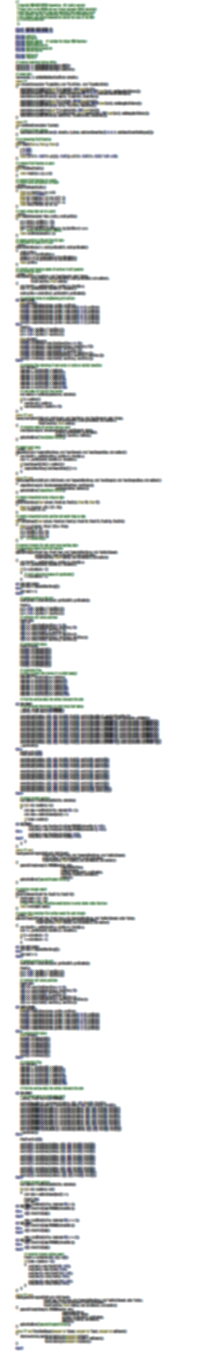
\includegraphics[width=.75in]{images/MCCompareCuda} &
    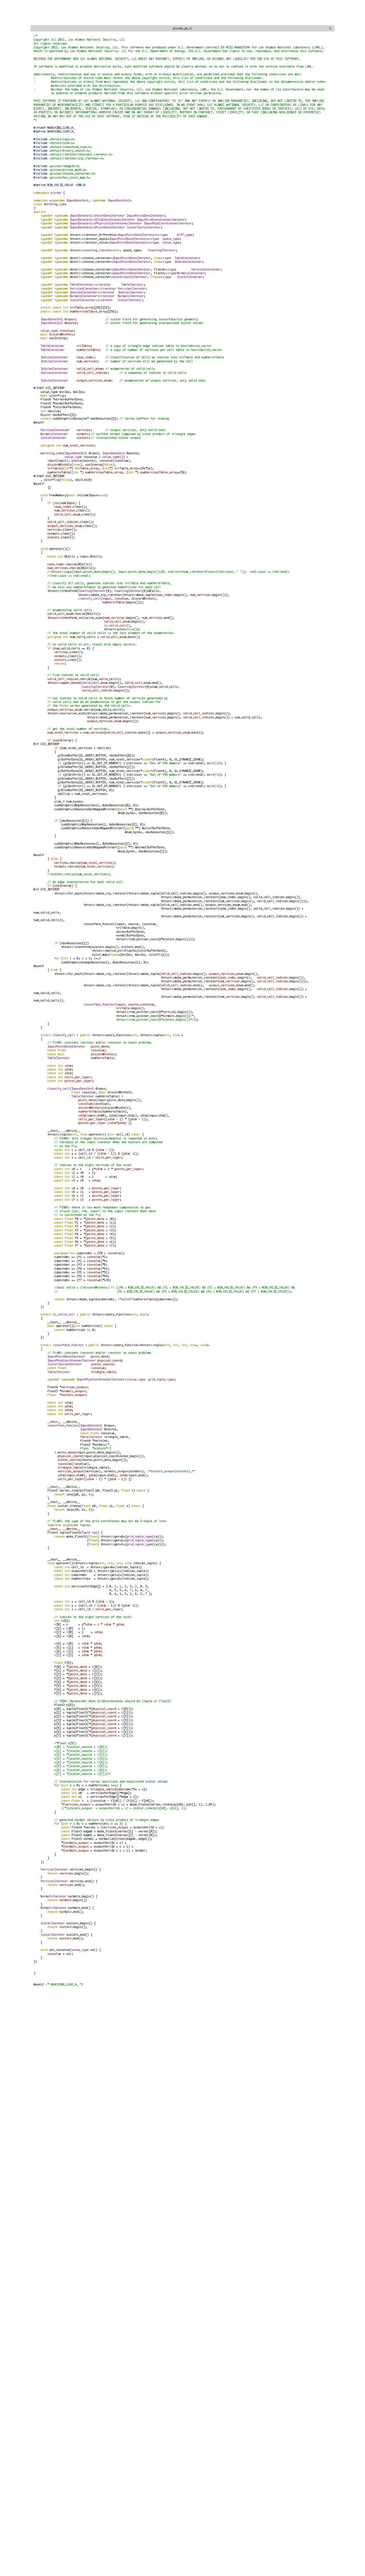
\includegraphics[width=.75in]{images/MCComparePiston} &
    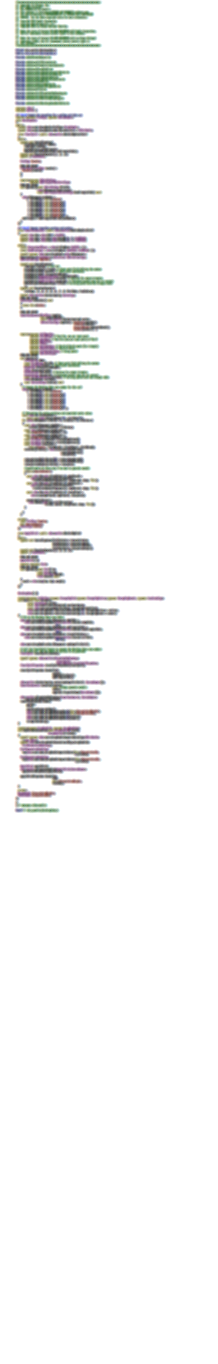
\includegraphics[width=.75in]{images/MCCompareVTKm}
  \end{tabular}
  \caption[Comparison of Marching Cubes implementations.]{Comparison of the
    Marching Cubes algorithm in VTK-m and two other implementations.
    Implementations in VTK-m are simpler, shorter, more general, and easier
    to maintain. (Lines of code (LOC) measurements come from cloc.}
  \label{fig:MCCompare}
\end{figure}

VTK-m simplifies the development of parallel scientific visualization
algorithms by providing a framework of supporting functionality that allows
developers to focus on visualization operations. Consider the listings in
Figure~\ref{fig:MCCompare} that compares the size of the implementations
for the Marching Cubes algorithm in VTK-m with the equivalent algorithms
implemented in the CUDA software development kit reference implementation
and the PISTON visualization library. Because VTK-m internally manages the
parallel distribution of work and data, the VTK-m implementation is shorter
and easier to maintain. Additionally, VTK-m provides data abstractions not
provided by the other libraries that make code written in VTK-m more
versatile.

\begin{didyouknow}
  VTK-m is written in C++ and makes extensive use of templates. The toolkit
  is implemented as a header library, meaning that all the code is
  implemented in header files (with extension \textfilename{.h}) and
  completely included in any code that uses it. This allows the compiler to
  inline and specialize code for better performance.
\end{didyouknow}

\section{How to Use This Guide}

This user's guide is organized into three parts to help guide novice to
advanced users and to provide a convenient reference.
Part~\ref{part:GettingStarted}, Getting Started, provides everything needed
to get up and running with VTK-m. In this part we learn the basics of
reading and writing data files, using filters to process data, and perform
basic rendering to view the results.

Part~\ref{part:Developing}, Developing with VTK-m, dives deeper into the
VTK-m library and provides all the information needed to customize VTK-m's
data structures and support multiple devices. Part~\ref{part:Developing}
also documents how to use VTK-m's framework to develop new or custom
visualization algorithms.

Part~\ref{part:Advanced}, Advanced Customization, exposes the inner
workings of VTK-m and allows you to design new algorithmic structures not
already available. \fix{This might be removed in the first version of the
  book.}

\section{Conventions Used in This Guide}

When documenting the VTK-m API, the following conventions are used.
\begin{itemize}
\item Filenames are printed in a \textfilename{sans serif font}.
\item C++ code is printed in a \textcode{monospace font}.
\item Macros and namespaces from VTK-m are printed in \textnamespace{red}.
\item Identifiers from VTK-m are printed in \textidentifier{blue}.
\item Signatures, described in Chapter~\ref{chap:Worklets}, and the
  tags used in them are printed in \textsignature{green}.
\end{itemize}

This guide provides actual code samples throughout its discussions to
demonstrate their use. These examples are all valid code that can be
compiled and used although it is often the case that code snippets are
provided. In such cases, the code must be placed in a larger context.

\begin{didyouknow}
  In this guide we periodically use these \textbf{Did you know?} boxes to
  provide additional information related to the topic at hand.
\end{didyouknow}

\begin{commonerrors}
  \textbf{Common Errors} blocks are used to highlight some of the common
  problems or complications you might encounter when dealing with the topic
  of discussion.
\end{commonerrors}


% -*- latex -*-

\chapter{Basic Provisions}
\label{chap:BasicProvisions}

This section describes the core facilities provided by VTK-m. These include
macros, types, and classes that define the environment in which code is
run, the core types of data stored, and template introspection. We also
start with a description of package structure used by VTK-m.


\section{General Approach}
\label{sec:GeneralApproach}

VTK-m is designed to provide a \keyterm{pervasive parallelism}
\index{pervasive parallelism} throughout all its visualization algorithms,
meaning that the algorithm is designed to operate with independent
concurrency at the finest possible level throughout. VTK-m provides this
pervasive parallelism by providing a programming construct called a
\keyterm{worklet}, \index{worklet} which operates on a very fine
granularity of data. The worklets are designed as serial components, and
VTK-m handles whatever layers of concurrency are necessary, thereby
removing the onus from the visualization algorithm developer. Worklet
operation is then wrapped into \keyterm{filters}, \index{filter} which
provide a simplified interface to end users.

A worklet is essentially a small functor \index{functor} or kernel
\index{kernel} designed to operate on a small element of data. (The name
``worklet'' means a small amount of work. We mean small in this sense to be
the amount of data, not necessarily the amount of instructions performed.)
The worklet is constrained to contain a serial and stateless function.
These constraints form three critical purposes. First, the constraints on
the worklets allow VTK-m to schedule worklet invocations on a great many
independent concurrent threads and thereby making the algorithm pervasively
parallel. Second, the constraints allow VTK-m to provide thread safety. By
controlling the memory access the toolkit can insure that no worklet will
have any memory collisions, false sharing, or other parallel programming
pitfalls. Third, the constraints encourage good programming practices. The
worklet model provides a natural approach to visualization algorithm design
that also has good general performance characteristics.

VTK-m allows developers to design algorithms that are run on massive
amounts of threads. However, VTK-m also allows developers to interface to
applications, define data, and invoke algorithms that they have written or
are provided otherwise. These two modes represent significantly different
operations on the data. The operating code of an algorithm in a worklet is
constrained to access only a small portion of data that is provided by the
framework. Conversely, code that is building the data structures needs to
manage the data in its entirety, but has little reason to perform
computations on any particular element.

Consequently, VTK-m is divided into two \keyterm{environments}
\index{environment} that handle each of these use cases. Each environment
has its own API, and direct interaction between the environments is
disallowed. The environments are as follows.

\begin{description}
\item[Execution Environment] \index{execution environment}
  \index{environment!execution} This is the environment in which the
  computational portion of algorithms are executed. The API for this
  environment provides work for one element with convenient access to
  information such as connectivity and neighborhood as needed by typical
  visualization algorithms. Code for the execution environment is designed
  to always execute on a very large number of threads.
\item[Control Environment] \index{control environment}
  \index{environment!control} This is the environment that is used to
  interface with applications, interface with I/O devices, and schedule
  parallel execution of the algorithms. The associated API is designed for
  users that want to use VTK-m to analyze their data using provided or
  supplied filters. Code for the control environment is designed to run on
  a single thread (or one single thread per process in an MPI job).
\end{description}

These dual programming environments are partially a convenience to isolate
the application from the execution of the worklets and are partially a
necessity to support GPU languages with host and device environments. The
control and execution environments are logically equivalent to the host and
device environments, respectively, in CUDA and other associated GPU
languages.

\begin{figure}[htb]
  \centering
  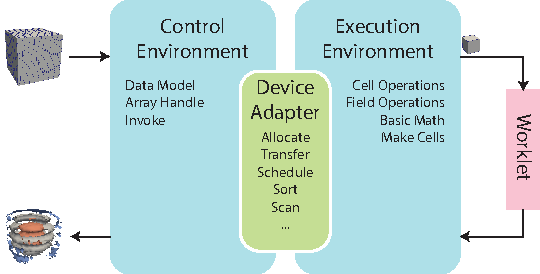
\includegraphics[width=4in]{images/VTKmEnvironments}
  \caption{Diagram of the VTK-m framework.}
  \label{fig:VTKmDiagram}
\end{figure}

Figure~\ref{fig:VTKmDiagram} displays the relationship between the control
and execution environment. The typical workflow when using VTK-m is that
first the control thread establishes a data set in the control environment
and then invokes a parallel operation on the data using a filter. From
there the data is logically divided into its constituent elements, which
are sent to independent invocations of a worklet. The worklet
invocations, being independent, are run on as many concurrent threads as
are supported by the device. On completion the results of the worklet
invocations are collected to a single data structure and a handle is
returned back to the control environment.

\begin{didyouknow}
  Are you only planning to use filters in VTK-m that already exist? If so,
  then everything you work with will be in the control environment. The
  execution environment is only used when implementing algorithms for
  filters.
\end{didyouknow}


\section{Package Structure}
\label{sec:PackageStructure}

\index{packages|(}

VTK-m is organized in a hierarchy of nested packages. VTK-m places
definitions in \keyterm{namespaces} \index{namespace} that correspond to
the package (with the exception that one package may specialize a template
defined in a different namespace).

The base package is named \vtkm{}. All classes within VTK-m are placed
either directly in the \vtkm{} package or in a package beneath it. This
helps prevent name collisions between VTK-m and any other library.

As described in Section~\ref{sec:GeneralApproach}, the VTK-m API is divided
into two distinct environments: \index{environment} the control environment
\index{control environment} \index{environment!control} and the execution
environment. \index{execution environment} \index{environment!execution}
The API for these two environments are located in the \vtkmcont{} and
\vtkmexec{} packages, respectively. Items located in the base \vtkm{}
namespace are available in both environments.

Although it is conventional to spell out names in identifiers (see the
coding conventions in Chapter~\ref{chap:CodingConventions}), there is an
exception to abbreviate control and execution to \textnamespace{cont}
and \textnamespace{exec}, respectively. This is because it is also part of
the coding convention to declare the entire namespace when using an
identifier that is part of the corresponding package. The shorter names
make the identifiers easier to read, faster to type, and more feasible to
pack lines in 80 column displays. These abbreviations are also used instead
of more common abbreviations (e.g. ctrl for control) because, as part of
actual English words, they are easier to type.

Further functionality in VTK-m is built on top of the base \vtkm{},
\vtkmcont{}, and \vtkmexec{} packages. Support classes for building
worklets, described in Chapter~\ref{chap:Worklets}, are contained in the
\vtkmworklet{} package. Other facilities in VTK-m are provided in their own
packages such as \vtkmio{}, \vtkmfilter{}, and \vtkmrendering{}. These
packages are described in Part~\ref{part:GettingStarted}.

VTK-m contains code that uses specialized compiler features, such as those
with CUDA, or libraries, such as Intel Threading Building Blocks, that will
not be available on all machines. Code for these features are encapsulated
in their own packages under the \vtkmcont{} namespace: \vtkmcontcuda{} and
\vtkmconttbb{}.

VTK-m contains OpenGL interoperability \index{OpenGL}
\index{interoperability} that allows data generated with VTK-m to be
efficiently transferred to OpenGL objects. This feature is encapsulated in
the \vtkmopengl{} package.

Figure~\ref{fig:Packages} provides a diagram of the VTK-m package hierarchy.

\begin{figure}[htb]
  \centering
  %% \begin{itemize}
  %% \item \vtkm{}
  %% \item \vtkmexec{}
  %% \item \vtkmcont{}
  %% \item \vtkmcontcuda{}
  %% \item \vtkmconttbb{}
  %% \item \vtkmio{}
  %% \item \vtkmioreader{}
  %% \item \vtkmiowriter{}
  %% \item \vtkmfilter{}
  %% \item \vtkmrendering{}
  %% \item \vtkmopengl{}
  %% \item \vtkmworklet{}
  %% %% \item \textnamespace{vtkm}
  %% %%   \begin{itemize}
  %% %%   \item \textnamespace{cont}
  %% %%   \item \textnamespace{exec}
  %% %%   \item \textnamespace{worklet}
  %% %%   \item \textnamespace{math}
  %% %%   \item \textnamespace{cuda}
  %% %%     \begin{itemize}
  %% %%     \item \textnamespace{cont}
  %% %%     \end{itemize}
  %% %%   \item \textnamespace{openmp}
  %% %%     \begin{itemize}
  %% %%     \item \textnamespace{cont}
  %% %%     \end{itemize}
  %% %%   \item \textnamespace{tbb}
  %% %%     \begin{itemize}
  %% %%     \item \textnamespace{cont}
  %% %%     \end{itemize}
  %% %%   \item \textnamespace{opengl}
  %% %%   \end{itemize}
  %% \end{itemize}
  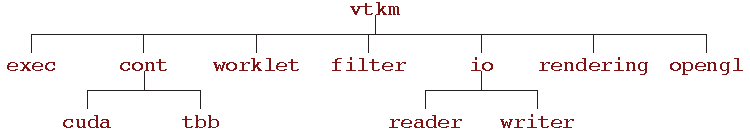
\includegraphics{images/PackageHierarchy}
  \caption{VTK-m package hierarchy.}
  \label{fig:Packages}
\end{figure}

By convention all classes will be defined in a file with the same name as
the class name (with a \textfilename{.h} extension) located in a directory
corresponding to the package name. For example, the \vtkmcont{ArrayHandle}
class is found in the \vtkmheader{vtkm/cont}{ArrayHandle.h} header. There
are, however, exceptions to this rule. Some smaller classes and types are
grouped together for convenience. These exceptions will be noted as
necessary.

Within each namespace there may also
be \textnamespace{internal}\indexnamespaceone{internal}
and \textnamespace{detail}\indexnamespaceone{detail}
sub-namespaces. The \textnamespace{internal} namespaces contain features
that are used internally and may change without
notice. The \textnamespace{detail} namespaces contain features that are
used by a particular class but must be declared outside of that
class. Users should generally ignore classes in these namespaces.

\index{packages|)}


\section{Function and Method Environment Modifiers}
\label{sec:FunctionAndMethodEnvironmentModifiers}

Any function or method defined by VTK-m must come with a modifier that determines in which environments the function may be run.
These modifiers are C macros that VTK-m uses to instruct the compiler for which architectures to compile each method.
Most user code outside of VTK-m need not use these macros with the important exception of any classes passed to VTK-m.
This occurs when defining new worklets, array storage, and device adapters.

VTK-m provides three modifier macros, \vtkmcontmodifier, \vtkmexecmodifier, and
\vtkmexeccontmodifier, which are used to declare functions and methods that
can run in the control environment, execution environment, and both
environments, respectively. These macros get defined by including just
about any VTK-m header file, but including \vtkmheader{vtkm}{Types.h} will
ensure they are defined. 

The modifier macro is placed after the template declaration, if there is one,
and before the return type for the function. Here is a simple example of a
function that will square a value. Since most types you would use this
function on have operators in both the control and execution environments,
the function is declared for both places.

\vtkmlisting{Usage of an environment modifier macro on a function.}{EnvironmentModifierMacro.cxx}

The primary function of the modifier macros is to inject compiler-specific
keywords that specify what architecture to compile code for. For example,
when compiling with CUDA\index{CUDA}, the control modifiers have
\textcode{\_\_host\_\_}\index{\_\_host\_\_} in them and execution modifiers
have \textcode{\_\_device\_\_}\index{\_\_device\_\_} in them.

There is one additional modifier macro that is not used for functions but
rather used when declaring a constant data object that is used in the
execution environment. This macro is named
\vtkmmacro{VTKM\_EXEC\_CONSTANT}\index{modifier!constant}\index{constant modifier}
and is used to declare a constant lookup table used when executing a
worklet. Its primary reason for existing is to add a
\textcode{\_\_constant\_\_} keyword when compiling with CUDA. This modifier
currently has no effect on any other compiler.

Finally, it is sometimes the case that a function declared as
\vtkmexeccontmodifier has to call a method declared as \vtkmexecmodifier or
\vtkmcontmodifier. Generally functions should not call other functions with
incompatible control/execution modifiers, but sometimes a generic
\vtkmexeccontmodifier function calls another function determined by the
template parameters, and the valid environments of this subfunction may be
inconsistent. For cases like this, you can use the
\vtkmmacro{VTKM\_SUPPRESS\_EXEC\_WARNINGS} to tell the compiler to ignore the
inconsistency when resolving the template. When applied to a templated
function or method, \vtkmmacro{VTKM\_SUPPRESS\_EXEC\_WARNINGS} is placed
before the \textcode{template} keyword. When applied to a non-templated
method in a templated class, \vtkmmacro{VTKM\_SUPPRESS\_EXEC\_WARNINGS} is
placed before the environment modifier macro.

\vtkmlisting{Suppressing warnings about functions from mixed environments.}{SuppressExecWarnings.cxx}


\section{Core Data Types}
\label{sec:CoreDataTypes}

Except in rare circumstances where precision is not a concern, VTK-m does
not directly use the core C types like \textcode{int}, \textcode{float},
and \textcode{double}. Instead, VTK-m provides its own core types, which
are declared in \vtkmheader{vtkm}{Types.h}.

\subsection{Single Number Types}

To ensure portability across different compilers and architectures, VTK-m
provides \textcode{typedef}s for the following basic types with explicit
precision: \vtkm{Float32}, \vtkm{Float64}, \vtkm{Int8}, \vtkm{Int16},
\vtkm{Int32}, \vtkm{Int64}, \vtkm{UInt8}, \vtkm{UInt16}, \vtkm{UInt32}, and
\vtkm{UInt64}. Under most circumstances when using VTK-m (and performing
visualization in general) the type of data is determined by the source of the
data or resolved through templates. In the case where a specific type of
data is required, these VTK-m--defined types should be preferred over basic
C types like \textcode{int} or \textcode{float}.

Many of the structures in VTK-m require indices to identify elements like
points and cells. All indices for arrays and other lists use the type
\vtkm{Id}. By default this type is a 32-bit wide integer but can be easily
changed by compile options. The CMake configuration option
\cmakevar{VTKM\_USE\_64BIT\_IDS} can be used to change \vtkm{Id} to be 64
bits wide. This configuration can be overridden by defining the C macro
\vtkmmacro{VTKM\_USE\_64BIT\_IDS} or \vtkmmacro{VTKM\_NO\_64BIT\_IDS} to
force \vtkm{Id} to be either 64 or 32 bits. These macros must be defined
before any VTK-m header files are included to take effect.

There is also a secondary index type named \vtkm{IdComponent} that is used
to index components of short vectors (discussed in
Section~\ref{sec:VectorTypes}). This type is an integer that might be a
shorter width than \vtkm{Id}.

There is also the rare circumstance in which an algorithm in VTK-m computes
data values for which there is no indication what the precision should
be. For these circumstances, the type \vtkm{FloatDefault} is provided. By
default this type is a 32-bit wide floating point number but can be easily
changed by compile options. The CMake configuration option
\cmakevar{VTKM\_USE\_DOUBLE\_PRECISION} can be used to change
\vtkm{FloatDefault} to be 64 bits wide. This configuration can be
overridden by defining the C macro \vtkmmacro{VTKM\_USE\_DOUBLE\_PRECISION}
or \vtkmmacro{VTKM\_NO\_DOUBLE\_PRECISION} to force \vtkm{FloatDefault} to
be either 64 or 32 bits. These macros must be defined before any VTK-m
header files are included to take
effect.

For convenience, you can include either
\vtkmheader{vtkm/internal}{ConfigureFor32.h} or
\vtkmheader{vtkm/internal}{ConfigureFor64.h} to force both \vtkm{Id} and
\vtkm{FloatDefault} to be 32 or 64 bits.

\subsection{Vector Types}
\label{sec:VectorTypes}

Visualization algorithms also often require operations on short vectors.
Arrays indexed in up to three dimensions are common. Data are often defined
in 2-space and 3-space, and transformations are typically done in
homogeneous coordinates of length 4. To simplify these types of operations,
VTK-m provides the \vtkm{Vec}\tparams{T,Size} templated type, which is
essentially a fixed length array of a given type.

The default constructor of \vtkm{Vec} objects leaves the values
uninitialized. All vectors have a constructor with one argument that is
used to initialize all components. All \vtkm{Vec} objects with a size of 4
or less is specialized to also have a constructor that allows you to set
the individual components. Likewise, there is a \vtkm{make\_Vec} function
that builds initialized vector types of up to 4 components. Once created,
you can use the bracket operator to get and set component values with the
same syntax as an array.

\vtkmlisting{Creating vector types.}{CreatingVectorTypes.cxx}

The types \vtkm{Id2} and \vtkm{Id3} are \textcode{typedef}s of
\vtkm{Vec}\tparams{\vtkm{Id},2} and \vtkm{Vec}\tparams{\vtkm{Id},2}. These
are used to index arrays of 2 and 3 dimensions, which is common.

Vectors longer than 4 are also supported, but independent component values must be set after construction.
The \vtkm{Vec} class contains a constant named \textidentifier{NUM\_COMPONENTS}\index{NUM\_COMPONENTS} to specify how many components are in the vector.
The class also has a \textcode{GetNumberOfComponents} method that also returns the number of components that are in the vector.

\vtkmlisting{A Longer Vector.}{LongerVector.cxx}

\vtkm{Vec} supports component-wise arithmetic using the operators
for plus (\textcode{+}), minus (\textcode{-}), multiply (\textcode{*}), and
divide (\textcode{/}). It also supports scalar to vector multiplication
with the multiply operator. The comparison operators equal (\textcode{==})
is true if every pair of corresponding components are true and not equal
(\textcode{!=}) is true otherwise. A special \vtkm{dot} function is
overloaded to provide a dot product for every type of vector.

\vtkmlisting{Vector operations.}{VectorOperations.cxx}

These operators, of course, only work if they are also defined for the
component type of the \vtkm{Vec}. For example, the multiply operator will
work fine on objects of type \vtkm{Vec}\tparams{char,3}, but the multiply
operator will not work on objects of type \vtkm{Vec}\tparams{std::string,3}
because you cannot multiply objects of type \textcode{std::string}.

In addition to generalizing vector operations and making arbitrarily long
vectors, \vtkm{Vec} can be repurposed for creating any sequence of
homogeneous objects. Here is a simple example of using \vtkm{Vec} to hold
the state of a polygon.

\vtkmlisting{Repurposing a \protect\vtkm{Vec}.}{EquilateralTriangle.cxx}

\index{Vec-like|(}

The \vtkm{Vec} class provides a convenient structure for holding and passing small vectors of data.
However, there are times when using \textidentifier{Vec} is inconvenient or inappropriate.
For example, the size of \vtkm{Vec} must be known at compile time, but there may be need for a vector whose size is unknown until compile time.
Also, the data populating a \vtkm{Vec} might come from a source that makes it inconvenient or less efficient to construct a \vtkm{Vec}.
For this reason, \VTKm also provides several \keyterm{\Veclike} objects that behave much like \vtkm{Vec} but are a different class.
These \Veclike objects have the same interface as \vtkm{Vec} except that the \textidentifier{NUM\_COMPONENTS} constant is not available on those that are sized at run time.
\Veclike objects also come with a \textcode{CopyInto} method that will take their contents and copy them into a standard \textidentifier{Vec} class.
(The standard \textidentifier{Vec} class also has a \textcode{CopyInto} method for consistency.)

The first \Veclike object is \vtkm{VecC}, which exposes a C-type array as a \textidentifier{Vec}.
The constructor for \vtkm{VecC} takes a C array and a size of that array.
There is also a constant version of \textidentifier{VecC} named \vtkm{VecCConst}, which takes a constant array and cannot be mutated.
The \vtkmheader{vtkm}{Types.h} header defines both \textidentifier{VecC} and \textidentifier{VecCConst} as well as multiple versions of \vtkm{make\_VecC} to easily convert a C array to either a \textidentifier{VecC} or \textidentifier{VecCConst}.

The following example demonstrates converting values from a constant table into a \vtkm{VecCConst} for further consumption.
The table and associated methods define how 8 points come together to form a hexahedron.

\vtkmlisting[ex:VecCConst]{Using \protect\vtkm{VecCConst} with a constant array.}{VecCExample.cxx}

\begin{commonerrors}
  The \vtkm{VecC} and \vtkm{VecCConst} classes only hold a pointer to a buffer that contains the data.
  They do not manage the memory holding the data.
  Thus, if the pointer given to \vtkm{VecC} or \vtkm{VecCConst} becomes invalid, then using the object becomes invalid.
  Make sure that the scope of the \vtkm{VecC} or \vtkm{VecCConst} does not outlive the scope of the data it points to.
\end{commonerrors}

The next \Veclike object is \vtkm{VecVariable}, which provides a \Veclike object that can be resized at run time to a maximum value.
Unlike \textidentifier{VecC}, \textidentifier{VecVariable} holds its own memory, which makes it a bit safer to use.
But also unlike \textidentifier{VecC}, you must define the maximum size of \textidentifier{VecVariable} at compile time.
Thus, \textidentifier{VecVariable} is really only appropriate to use when there is a predetermined limit to the vector size that is fairly small.

The following example uses a \vtkm{VecVariable} to store the trace of edges within a hexahedron.
This example uses the methods defined in Example~\ref{ex:VecCConst}.

\vtkmlisting{Using \protect\vtkm{VecVariable}.}{VecVariableExample.cxx}

\VTKm provides further examples of \Veclike objects as well.
For example, the \vtkm{VecFromPortal} and \vtkm{VecFromPortalPermute} objects allow you to treat a subsection of an arbitrarily large array as a \textidentifier{Vec}.
These objects work by attaching to array portals, which are described in Section~\ref{sec:ArrayPortals}.
Another example of a \Veclike object is \vtkm{VecRectilinearPointCoordinates}, which efficiently represents the point coordinates in an axis-aligned hexahedron.
Such shapes are common in structured grids.
These and other data sets are described in Chapter~\ref{chap:DataSets}.

\index{Vec-like|)}


\subsection{Pair}
\label{sec:Pair}

VTK-m defines a \vtkm{Pair}\tparams{T1,T2} templated object that
behaves just like \textcode{std:\colonhyp{}pair} from the standard template
library. The difference is that \vtkm{Pair} will work in both the execution
and control environment, whereas the STL \textcode{std::pair} does not
always work in the execution environment.

The VTK-m version of \vtkm{Pair} supports the same types, fields, and
operations as the STL version. VTK-m also provides a \vtkm{make\_Pair}
function for convenience.

\subsection{Range}
\label{sec:Range}

VTK-m provides a convenience structure named \vtkm{Range} to help manage a
range of values. The \textidentifier{Range} \textcode{struct} contains two
data members, \textcode{Min} and \textcode{Max}, which represent the ends
of the range of numbers. \textcode{Min} and \textcode{Max} are both of type
\vtkm{Float64}. \textcode{Min} and \textcode{Max} can be directly accessed,
but \textidentifier{Range} also comes with the following helper functions
to make it easier to build and use ranges. Note that all of these functions
treat the minimum and maximum value as inclusive to the range.

\begin{description}
\item[\textcode{IsNonEmpty}] Returns true if the range covers at least one
  value.
\item[\textcode{Contains}] Takes a single number and returns true if that
  number is contained within the range.
\item[\textcode{Length}] Returns the distance between \textcode{Min} and
  \textcode{Max}. Empty ranges return a length of 0. Note that if the range
  is non-empty and the length is 0, then \textcode{Min} and \text{Max} must
  be equal, and the range contains exactly one number.
\item[\textcode{Center}] Returns the number equidistant to \textcode{Min}
  and \textcode{Max}. If the range is empty, NaN is returned.
\item[\textcode{Include}] Takes either a single number or another range and
  modifies this range to include the given number or range. If necessary,
  the range is grown just enough to encompass the given argument. If the
  argument is already in the range, nothing changes.
\item[\textcode{Union}] A nondestructive version of \textcode{Include},
  which builds a new \textidentifier{Range} that is the union of this range
  and the argument. The \textcode{+} operator is also overloaded to compute
  the union.
\end{description}

The following example demonstrates the operation of \vtkm{Range}.

\vtkmlisting{Using \protect\vtkm{Range}.}{UsingRange.cxx}

\subsection{Bounds}
\label{sec:Bounds}

VTK-m provides a convenience structure named \vtkm{Bounds} to help manage
an axis-aligned region in 3D space. Among other things, this structure is
often useful for representing a bounding box for geometry. The
\textidentifier{Bounds} \textcode{struct} contains three data members,
\textcode{X}, \textcode{Y}, and \textcode{Z}, which represent the range of
the bounds along each respective axis. All three of these members are of
type \vtkm{Range}, which is discussed previously in
Section~\ref{sec:Range}. \textcode{X}, \textcode{Y}, and \textcode{Z} can
be directly accessed, but \textidentifier{Bounds} also comes with the
following helper functions to make it easier to build and use ranges.

\begin{description}
\item[\textcode{IsNonEmpty}] Returns true if the bounds cover at least one
  value.
\item[\textcode{Contains}] Takes a \vtkm{Vec} of size 3 and returns true if
  those point coordinates are contained within the range.
\item[\textcode{Center}] Returns the point at the center of the range as a
  \vtkm{Vec}\textcode{<}\vtkm{Float64}\textcode{,3>}.
\item[\textcode{Include}] Takes either a \vtkm{Vec} of size 3 or another
  bounds and modifies this bounds to include the given point or bounds. If
  necessary, the bounds are grown just enough to encompass the given
  argument. If the argument is already in the bounds, nothing changes.
\item[\textcode{Union}] A nondestructive version of \textcode{Include},
  which builds a new \textidentifier{Bounds} that is the union of this
  bounds and the argument. The \textcode{+} operator is also overloaded to
  compute the union.
\end{description}

The following example demonstrates the operation of \vtkm{Bounds}.

\vtkmlisting{Using \protect\vtkm{Bounds}.}{UsingBounds.cxx}


\section{Traits}
\label{sec:Traits}

\index{traits|(}

When using templated types, it is often necessary to get information about
the type or specialize code based on general properties of the type. VTK-m
uses traits classes to publish and retrieve information about types. A
traits class is simply a templated structure that provides typedefs for
tag\index{tag} structures, empty types used for identification. The traits
classes might also contain constant numbers and helpful static
functions. See {\it Effective C++ Third Edition} by Scott Mayers for a
description of traits classes and their uses.

\subsection{Type Traits}

\index{traits!type|(}
\index{type traits|(}

The \vtkm{TypeTraits}\tparams{T} templated class provides basic information
about a core type. These type traits are available for all the basic C++
types as well as the core VTK-m types described in
Section~\ref{sec:CoreDataTypes}. \vtkm{TypeTraits} contains the following
elements.

\index{tag!type traits|(}

\begin{description}
\item[\textidentifier{NumericTag}] \index{NumericTag} \index{tag!numeric}
  This type is set to either \vtkm{TypeTraitsRealTag} or
  \vtkm{TypeTraitsIntegerTag} to signal that the type represents either
  floating point numbers or integers.
\item[\textidentifier{DimensionalityTag}] \index{DimensionalityTag}
  \index{tag!dimensionality} This type is set to either
  \vtkm{TypeTraitsScalarTag} or \vtkm{TypeTraitsVectorTag} to signal that
  the type represents either a single scalar value or a tuple of values.
\item[\textidentifier{ZeroInitialization}] \index{ZeroInitialization}
  A static member function that takes no arguments and returns 0 (or the closest equivalent to it) cast to the type.
\end{description}

The definition of \vtkm{TypeTraits} for \vtkm{Float32} could like something
like this.
\vtkmlisting{Definition of \protect \vtkm{TypeTraits}\tparams{\protect \vtkm{Float32}}.}{TypeTraitsImpl.cxx}

Here is a simple example of using \vtkm{TypeTraits} to implement a generic
function that behaves like the remainder operator (\textcode{\%}) for all
types including floating points and vectors.

\vtkmlisting[ex:TypeTraits]{Using \textidentifier{TypeTraits} for a generic remainder.}{TypeTraits.cxx}

\index{tag!type traits|)}

\index{type traits|)}
\index{traits!type|)}


\subsection{Vector Traits}
\label{sec:VectorTraits}

\index{traits!vector|(}
\index{vector traits|(}

The templated \vtkm{Vec} class contains several items for introspection (such as the component type and its size).
However, there are other types behave similarly to \textidentifier{Vec} objects but have different ways to perform this introspection.
\index{Vec-like} For example, \VTKm contains \Veclike objects that essentially behave the same but might have different features such as a variable number of components.
Also, there may be reason to interchangeably use basic scalar values, like an integer or floating point number, with vectors.

To provide a consistent interface to access these multiple types that represents vectors, the \vtkm{VecTraits}\tparams{T} templated class provides information and accessors to vector types.
It contains the following elements.

\index{tag!vector traits|(}

\begin{description}
\item[\textidentifier{ComponentType}]
  \index{ComponentType}
  This type is set to the type for each component in the vector.
  For example, a \vtkm{Id3} has \textidentifier{ComponentType} defined as \vtkm{Id}.
\item[\textidentifier{IsSizeStatic}]
  \index{IsSizeStatic} \index{tag!static vector size} \index{tag!variable vector size}
  This type is set to either \vtkm{VecTraitsTagSizeStatic} if the vector has a static number of components that can be determined at compile time or set to \vtkm{VecTraitsTagSizeVariable} if the size of the vector is determined at run time.
  If \textidentifier{IsSizeStatic} is set to \textidentifier{VecTraitsTagSizeVariable}, then \textidentifier{VecTraits} will be missing some information that cannot be determined at compile time.
\item[\textidentifier{HasMultipleComponents}]
  \index{HasMultipleComponents} \index{tag!single component} \index{tag!multiple components}
  This type is set to either \vtkm{VecTraitsTagSingleComponent} if the vector length is size 1 or \vtkm{VecTraitsTagMultipleComponents} otherwise.
  This tag can be useful for creating specialized functions when a vector is really just a scalar.
  If the vector type is of variable size (that is, \textidentifier{IsSizeStatic} is \textidentifier{VecTraitsTagSizeVariable}), then \textidentifier{HasMultipleComponents} might be \textidentifier{VecTraitsTagMultipleComponents} even when at run time there is only one component.
\item[\textidentifier{NUM\_COMPONENTS}] \index{NUM\_COMPONENTS}
  An integer specifying how many components are contained in the vector.
  \textidentifier{NUM\_COMPONENTS} is not available for vector types of variable size (that is, \textidentifier{IsSizeStatic} is \textidentifier{VecTraitsTagSizeVariable}).
\item[\textcode{GetNumberOfComponents}] \index{GetNumberOfComponents}
  A static method that takes an instance of a vector and returns the number of components the vector contains.
  The result of \textcode{GetNumberOfComponents} is the same value of \textidentifier{NUM\_COMPONENTS} for vector types that have a static size (that is, \textidentifier{IsSizeStatic} is \textidentifier{VecTraitsTagSizeStatic}).
  But unlike \textidentifier{NUM\_COMPONENTS}, \textcode{GetNumberOfComponents} works for vectors of any type.
\item[\textcode{GetComponent}] \index{GetComponent}
  A static method that takes a vector and returns a particular component.
\item[\textcode{SetComponent}] \index{SetComponent}
  A static method that takes a vector and sets a particular component to a given value.
\item[\textcode{CopyInto}] \index{CopyInto}
  A static method that copies the components of a vector to a \vtkm{Vec}.
\end{description}

The definition of \vtkm{VecTraits} for \vtkm{Id3} could look something like
this.
\vtkmlisting{Definition of \protect \vtkm{VecTraits}\tparams{\protect \vtkm{Id3}}.}{VecTraitsImpl.cxx}

\index{tag!vector traits|)}

The real power of vector traits is that they simplify creating generic
operations on any type that can look like a vector. This includes
operations on scalar values as if they were vectors of size one. The
following code uses vector traits to simplify the implementation of less
functors\index{less} that define an ordering that can be used for sorting
and other operations.

\vtkmlisting{Using \textidentifier{VecTraits} for less functors.}{VecTraits.cxx}

\index{vector traits|)}
\index{traits!vector|)}

\index{traits|)}


\section{List Tags}
\label{sec:ListTags}

\index{tag!lists|(}
\index{lists|(}

\index{template metaprogramming}
\index{metaprogramming}
VTK-m internally uses template metaprogramming, which utilizes C++
templates to run source-generating programs, to customize code to various
data and compute platforms. One basic structure often uses with template
metaprogramming is a list of class names (also sometimes called a tuple or
vector, although both of those names have different meanings in VTK-m).

Many VTK-m users only need predefined lists, such as the type lists
specified in Section~\ref{sec:TypeLists}. Those users can skip most of the
details of this section. However, it is sometimes useful to modify lists,
create new lists, or operate on lists, and these usages are documented
here.

VTK-m uses a tag-based mechanism for defining lists, which differs
significantly from lists in many other template metaprogramming libraries
such as with \textcode{boost:\colonhyp{}mpl:\colonhyp{}vector} or
\textcode{boost:\colonhyp{}vector}. Rather than enumerating all list
entries as template arguments, the list is referenced by a single tag class
with a descriptive name. The intention is to make fully resolved types
shorter and more readable. (Anyone experienced with template programming
knows how insanely long and unreadable types can get in compiler errors and
warnings.)

\subsection{Building List Tags}
\label{sec:BuildingListTags}

List tags are constructed in VTK-m by defining a \textcode{struct} that
publicly inherits from another list tags. The base list tags are defined in
the \vtkmheader{vtkm}{ListTag.h} header.

The most basic list is defined with \vtkm{ListTagEmpty}. This tag
represents an empty list.

\vtkm{ListTagBase}\tparams{T, ...} represents a list of the types given as
template parameters. \vtkm{ListTagBase} supports a variable number of
parameters with the maximum specified by \vtkmmacro{VTKM\_MAX\_BASE\_LIST}.

Finally, lists can be combined together with
\vtkm{ListTagJoin}\tparams{ListTag1,ListTag2}, which concatinates two lists
together.

The following example demonstrates how to build list tags using these base
lists classes. Note first that all the list tags are defined as
\textcode{struct} rather than \textcode{class}. Although these are roughly
synonymous in C++, \textcode{struct} inheritance is by default public, and
public inheritance is important for the list tags to work. Note second that
these tags are created by inheritance rather than using
\textcode{typedef}. Although \textcode{typedef} will work, it will lead to
much uglier type names defined by the compiler.

\vtkmlisting{Creating list tags.}{BaseListTags.cxx}

\subsection{Type Lists}
\label{sec:TypeLists}

\index{type lists|(}
\index{lists!types|(}
\index{tag!type lists|(}

One of the major use cases for template metaprogramming lists in VTK-m is
to identify a set of potential data types for arrays. The
\vtkmheader{vtkm}{TypeListTag.h} header contains predefined lists for known
VTK-m types. Although technically all these lists are of C++ types, the
types we refer to here are those data types stored in data arrays. The
following lists are provided.

\begin{description}
\item[\vtkm{TypeListTagId}] Contains the single item \vtkm{Id}.
\item[\vtkm{TypeListTagId2}] Contains the single item \vtkm{Id2}.
\item[\vtkm{TypeListTagId3}] Contains the single item \vtkm{Id3}.
\item[\vtkm{TypeListTagIndex}] A list of all types used to index
  arrays. Contains \vtkm{Id}, \vtkm{Id2}, and \vtkm{Id3}.
\item[\vtkm{TypeListTagFieldScalar}] A list containing types used for
  scalar fields. Specifically, it contains floating point numbers of
  different widths (i.e. \vtkm{Float32} and \vtkm{Float64}).
\item[\vtkm{TypeListTagFieldVec2}] A list containing types for values of
  fields with 2 dimensional vectors. All these vectors use floating point
  numbers.
\item[\vtkm{TypeListTagFieldVec3}] A list containing types for values of
  fields with 3 dimensional vectors. All these vectors use floating point
  numbers.
\item[\vtkm{TypeListTagFieldVec3}] A list containing types for values of
  fields with 3 dimensional vectors. All these vectors use floating point
  numbers.
\item[\vtkm{TypeListTagField}] A list containing all the types generally
  used for fields. It is the combination of \vtkm{TypeListTagFieldScalar},
  \vtkm{TypeListTagFieldVec2}, \vtkm{TypeListTagFieldVec3}, and
  \vtkm{TypeListTagFieldVec4}.
\item[\vtkm{TypeListTagScalarAll}] A list of all scalar types. It contains
  signed and unsigned integers of widths from 8 to 64 bits. It also
  contains floats of 32 and 64 bit widths.
\item[\vtkm{TypeListTagVecCommon}] A list of the most common vector
  types. It contains all \vtkm{Vec} class of size 2 through 4 containing
  components of unsigned bytes, signed 32-bit integers, signed 64-bit
  integers, 32-bit floats, or 64-bit floats.
\item[\vtkm{TypeListTagVecAll}] A list of all \vtkm{Vec} classes with
  standard integers or floating points as components and lengths between 2
  and 4.
\item[\vtkm{TypeListTagAll}] A list of all types included in
  \vtkmheader{vtkm}{Types.h} with \vtkm{Vec}s with up to 4 components.
\item[\vtkm{TypeListTagCommon}] A list containing only the most used types
  in visualization. This includes signed integers and floats that are 32 or
  64 bit. It also includes 3 dimensional vectors of floats. This is the
  default list used when resolving the type in dynamic arrays (described in
  Chapter~\ref{chap:DynamicArrayHandle}).
\end{description}

If these lists are not sufficient, it is possible to build new type lists
using the existing type lists and the list bases from
Section~\ref{sec:BuildingListTags} as demonstrated in the following
example.

\vtkmlisting[ex:CustomTypeLists]{Defining new type lists.}{CustomTypeLists.cxx}

The \vtkmheader{vtkm}{TypeListTag.h} header also defines a macro named
\vtkmmacro{VTKM\_DEFAULT\_TYPE\_LIST\_TAG} that defines a default list of
types to use in classes like \vtkmcont{DynamicArrayHandle}
(Chapter~\ref{chap:DynamicArrayHandle}). This list can be overridden by
defining the \vtkmmacro{VTKM\_DEFAULT\_TYPE\_LIST\_TAG} macro \emph{before}
any VTK-m headers are included. If included after a VTK-m header, the list
is not likely to take effect. Do not ignore compiler warnings about the
macro being redefined, which you will not get if defined
correctly. Example~\ref{ex:CustomTypeLists} also contains an example of
overriding the \vtkmmacro{VTKM\_DEFAULT\_TYPE\_LIST\_TAG} macro.

\index{tag!type lists|)}
\index{lists!types|)}
\index{type lists|)}

\subsection{Operating on Lists}
\label{sec:OperatingOnLists}

VTK-m template metaprogramming lists are typically just passed to VTK-m
methods that internally operate on the lists. Although not typically used
outside of the VTK-m library, these operations are also available.

The \vtkmheader{vtkm}{ListTag.h} header comes with a \vtkm{ListForEach}
function that takes a functor object and a list tag. It then calls the
functor object with the default object of each type in the list. This is
most typically used with C++ run-time type information to convert a
run-time polymorphic object to a statically typed (and possibly inlined)
call.

The following example shows a rudimentary version of coverting a
dynamically-typed array to a statically-typed array similar to what is done
in VTK-m classes like \vtkmcont{DynamicArrayHandle} (which is documented in
Chapter~\ref{chap:DynamicArrayHandle}).

\vtkmlisting{Converting dynamic types to static types with \textidentifier{ListForEach}.}{ListForEach.cxx}

\index{lists|)}
\index{tag!lists|)}


\section{Error Handling}
\label{sec:ErrorHandlingControl}

\index{errors|(}

\index{errors!control environment|(}

VTK-m uses exceptions to report errors. All exceptions thrown by VTK-m will
be a subclass of \vtkmcont{Error}. For simple error reporting, it is
possible to simply catch a \vtkmcont{Error} and report the error message
string reported by the \textcode{GetMessage} method.

\vtkmlisting{Simple error reporting.}{CatchingErrors.cxx}

There are several subclasses to \vtkmcont{Error}. The specific subclass
gives an indication of the type of error that occured when the exception
was thrown. Catching one of these subclasses may help a program better
recover from errors.
\begin{description}
\item[\vtkmcont{ErrorBadAllocation}] Thrown when there is a problem
  accessing or manipulating memory. Often this is thrown when an allocation
  fails because there is insufficient memory, but other memory access
  errors can cause this to be thrown as well.
\item[\vtkmcont{ErrorBadType}] Thrown when VTK-m attempts to perform
  an operation on an object that is of an incompatible type.
\item[\vtkmcont{ErrorBadValue}] Thrown when a VTK-m function or
  method encounters an invalid value that inhibits progress.
\item[\vtkmcont{ErrorExecution}] \index{errors!execution environment} Throw
  when an error is signaled in the execution environment for example when a
  worklet is being executed.
\item[\vtkmcont{ErrorInternal}] Thrown when VTK-m detects an
  internal state that should never be reached. This error usually indicates
  a bug in VTK-m or, at best, VTK-m failed to detect an invalid input it
  should have.
\item[\vtkmio{ErrorIO}] Thrown by a reader or writer when a file error is
  encountered.
\end{description}

\index{errors!control environment|)}

\index{assert|(}
\index{errors!assert|(}

In addition to the aforementioned error signaling, the
\vtkmheader{vtkm}{Assert.h} header file defines a macro named
\vtkmmacro{VTKM\_ASSERT}. This macro behaves the same as the POSIX
\textmacro{assert} macro. It takes a single argument that is a condition
that is expected to be true. If it is not true, the program is halted and a
message is printed. Asserts are useful debugging tools to ensure that
software is behaving and being used as expected.

\vtkmlisting{Using \protect\vtkmmacro{VTKM\_ASSERT}.}{Assert.cxx}

\begin{didyouknow}
  Like the POSIX \textmacro{assert}, if the \vtkmmacro{NDEBUG} macro is
  defined, then \vtkmmacro{VTKM\_ASSERT} will become an empty expression.
  Typically \vtkmmacro{NDEBUG} is defined with a compiler flag (like
  \textcode{-DNDEBUG}) for release builds to better optimize the code.
  CMake will automatically add this flag for release builds.
\end{didyouknow}

\begin{commonerrors}
  A helpful warning provided by many compilers alerts you of unused
  variables. (This warning is commonly enabled on VTK-m regression test
  nightly builds.) If a function argument is used only in a
  \vtkmmacro{VTKM\_ASSERT}, then it will be required for debug builds and
  be unused in release builds. To get around this problem, add a statement
  to the function of the form \textcode{(void)\textit{variableName};}. This
  statement will have no effect on the code generated but will suppress the
  warning for release builds.
\end{commonerrors}

\index{assert!static|(}
\index{static assert|(}

Because \VTKm makes heavy use of C++ templates, it is possible that these templates could be used with inappropriate types in the arguments.
Using an unexpected type in a template can lead to very confusing errors, so it is better to catch such problems as early as possible.
The \vtkmmacro{VTKM\_STATIC\_ASSERT} macro, defined in \vtkmheader{vtkm}{StaticAssert.h} makes this possible.
This macro takes a constant expression that can be evaluated at compile time and verifies that the result is true.

In the following example, \vtkmmacro{VTKM\_STATIC\_ASSERT} and its sister macro \vtkmmacro{VTKM\_STATIC\_ASSERT\_MSG}, which allows you to give a descriptive message for the failure, are used to implement checks on a templated function that is designed to work on any scalar type that is represented by 32 or more bits.

\vtkmlisting[ex:StaticAssert]{Using \protect\vtkmmacro{VTKM\_STATIC\_ASSERT}.}{StaticAssert.cxx}

\begin{didyouknow}
  \index{is\_same}
  In addition to the several trait template classes provided by \VTKm to introspect C++ types, the C++ standard \textfilename{type\_traits} header file contains several helpful templates for general queries on types.
  Example~\ref{ex:StaticAssert} demonstrates the use of one such template: \textcode{std::is\_same}.
\end{didyouknow}

\begin{commonerrors}
  \index{true\_type} \index{false\_type} \index{type\_traits}
  Many templates used to introspect types resolve to the tags \textcode{std::true\_type} and \textcode{std::false\_type} rather than the constant values \textcode{true} and \textcode{false} that \vtkmmacro{VTKM\_STATIC\_ASSERT} expects.
  The \textcode{std::true\_type} and \textcode{std::false\_type} tags can be converted to the Boolean literal by adding \textcode{::value} to the end of them.
  Failing to do so will cause \vtkmmacro{VTKM\_STATIC\_ASSERT} to behave incorrectly.
  Example~\ref{ex:StaticAssert} demonstrates getting the Boolean literal from the result of \textcode{std::is\_same}.
\end{commonerrors}

\index{static assert|)}
\index{assert!static|)}

\index{errors!assert|)}
\index{assert|)}

\index{errors|)}


\section{\VTKm Version}
\label{sec:Version}

\index{version|(}

As the \VTKm code evolves, changes to the interface and behavior will inevitably happen.
Consequently, code that links into \VTKm might need a specific version of \VTKm or changes its behavior based on what version of \VTKm it is using.
To facilitate this, \VTKm software is managed with a versioning system and advertises its version in multiple ways.
As with many software products, \VTKm has three version numbers: major, minor, and patch.
The major version represents significant changes in the \VTKm implementation and interface.
Changes in the major version include backward incompatible changes.
The minor version represents added functionality.
Generally, changes in the minor version to not introduce changes to the API (although the early 1.X versions of \VTKm violate this).
The patch version represents fixes provided after a release occurs.
Patch versions represent minimal change and do not add features.

\index{version!CMake|(}
\index{CMake|(}
\index{CMake!version|(}
\index{CMake!VTK-m package!version|(}
\index{VTK-m CMake package!version|(}

If you are writing a software package that is managed by CMake and load \VTKm with the \textcode{find\_package} command as described in Section~\ref{sec:LinkingToVTKm}, then you can query the \VTKm version directly in the CMake configuration.
When you load \VTKm with \textcode{find\_package}, CMake sets the variables \cmakevar{VTKm\_VERSION\_MAJOR}, \cmakevar{VTKm\_VERSION\_MINOR}, and \cmakevar{VTKm\_VERSION\_PATCH} to the major, minor, and patch versions, respectively.
Additionally, \cmakevar{VTKm\_VERSION} is set to the ``major.minor'' version number and \cmakevar{VTKm\_VERSION\_FULL} is set to the ``major.minor.patch'' version number.
If the current version of \VTKm is actually a development version that is in between releases of \VTKm, then and abbreviated SHA of the git commit is also included as part of \cmakevar{VTKm\_VERSION\_FULL}.

\begin{didyouknow}
  If you have a specific version of \VTKm required for your software, you can also use the version option to the \textcode{find\_package} CMake command.
  The \textcode{find\_package} command takes an optional version argument that causes the command to fail if the wrong version of the package is found.
\end{didyouknow}

\index{VTK-m CMake package!version|)}
\index{CMake!VTK-m package!version|)}
\index{CMake!version|)}
\index{CMake|)}
\index{version!CMake|)}

\index{version!macro|(}

It is also possible to query the \VTKm version directly in your code through preprocessor macros.
The \vtkmheader{vtkm}{Version.h} header file defines the following preprocessor macros to identify the \VTKm version.
\vtkmmacro{VTKM\_VERSION\_MAJOR}, \vtkmmacro{VTKM\_VERSION\_MINOR}, and \vtkmmacro{VTKM\_VERSION\_PATCH} are set to integer numbers representing the major, minor, and patch versions, respectively.
Additionally, \vtkmmacro{VTKM\_VERSION} is set to the ``major.minor'' version number as a string and \vtkmmacro{VTKM\_VERSION\_FULL} is set to the ``major.minor.patch'' version number (also as a string).
If the current version of \VTKm is actually a development version that is in between releases of \VTKm, then and abbreviated SHA of the git commit is also included as part of \vtkmmacro{VTKM\_VERSION\_FULL}.

\begin{commonerrors}
  Note that the CMake variables all begin with \textcode{VTKm\_} (lowercase ``m'') whereas the preprocessor macros begin with \textcode{VTKM\_} (all uppercase).
  This follows the respective conventions of CMake variables and preprocessor macros.
\end{commonerrors}

Note that \vtkmheader{vtkm}{Version.h} does not include any other \VTKm header files.
This gives your code a chance to load, query, and react to the \VTKm version before loading any \VTKm code proper.

\index{version!macro|)}

\index{version|)}


\chapter{Provided Worklets}
\label{chap:ProvidedWorklets}

\fix{Write this once some worklets are provided. I expect before this we
  will have a chapter on provided filters. In fact, that probably means
  this chapter should move after the chapters on control and execution
  environments.}

\chapter{Control Environment}
\label{chap:ControlEnvironment}

\fix{Write this.}

\chapter{Execution Environment}
\label{chap:ExecutionEnvironment}

\fix{Write this.}

\chapter{OpenGL Interoperability}
\label{chap:OpenGLInteroperability}

\chapter{Coding Conventions}
\label{chap:CodingConventions}


\begin{flushleft}
  \clearpage
  \lhead[]{}
  \rhead[]{}
  \phantomsection
  \addcontentsline{toc}{chapter}{Index}
  \printindex
\end{flushleft}

% -*- latex -*-

\begin{SANDdistribution}[NM]
  % External Addresses
  %% \SANDdistExternal{1}{Lucy Nowell\\ U.S. Department of Energy\\ SC-21\\ 19901 Germantown Road\\ Germantown, MD 20874-1290}
  %% \SANDdistExternal{1}{Teresa Beachley\\ U.S. Department of Energy\\ SC-21\\ 19901 Germantown Road\\ Germantown, MD 20874-1290}
  %% \SANDdistExternal{1}{Berk Geveci\\ Kitware, Inc.\\ 28 Corporate Drive\\ Clifton Park, NY 12065}
  %% \SANDdistExternal{1}{Robert Maynard\\ Kitware, Inc.\\ 28 Corporate Drive\\ Clifton Park, NY 12065}
  %% \SANDdistExternal{1}{Kwan-Liu Ma\\ Department of Computer Science\\ 2063 Kemper Hall\\ University of California-Davis\\ One Shields Avenue\\ Davis, CA 95616-8562}

  \bigskip

  % Internal Addresses
  \SANDdistInternal{1}{1326}{Kenneth Moreland}{1461}
  \SANDdistInternal{1}{1327}{Ron Oldfield}{01461}
\end{SANDdistribution}


\end{document}
